\section{Experimental Results}
\label{sec:experiment}

We synthesized implementations for 46 Lustre models%
\footnote{The models are part of a larger collection
that can be found at
https://tinyurl.com/gt4geqz}~\cite{Hagen08:FMCAD}, including the running example from Fig.~\ref{fg:example}.
 The original models already contained an implementation,
which provided us with a complete test benchmark suite, since we were able to
compare the synthesized implementations to handwritten programs.
We compared the C implementations by \jkindsynt against the original models, after they had been translated
to C using the \lustrev compiler~\cite{lustrev6}.

% \begin{figure}[]
% 	\centering
% 	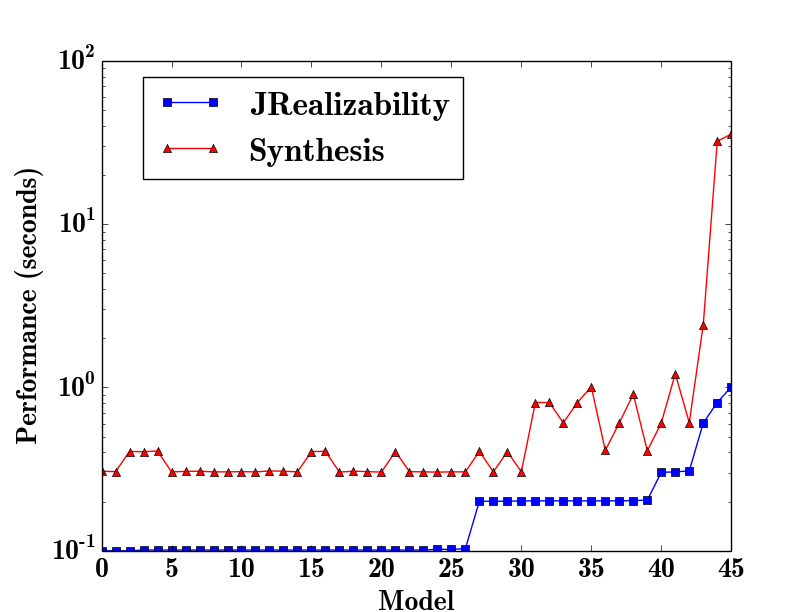
\includegraphics[width=0.6\textwidth,height=\textheight,keepaspectratio]{overhead}    	
% 	\caption{Overhead of synthesis to realizability checking}
% 	\label{fg:overhead}
% \end{figure}


\begin{figure}[h!]
	\centering
	\subfloat[]{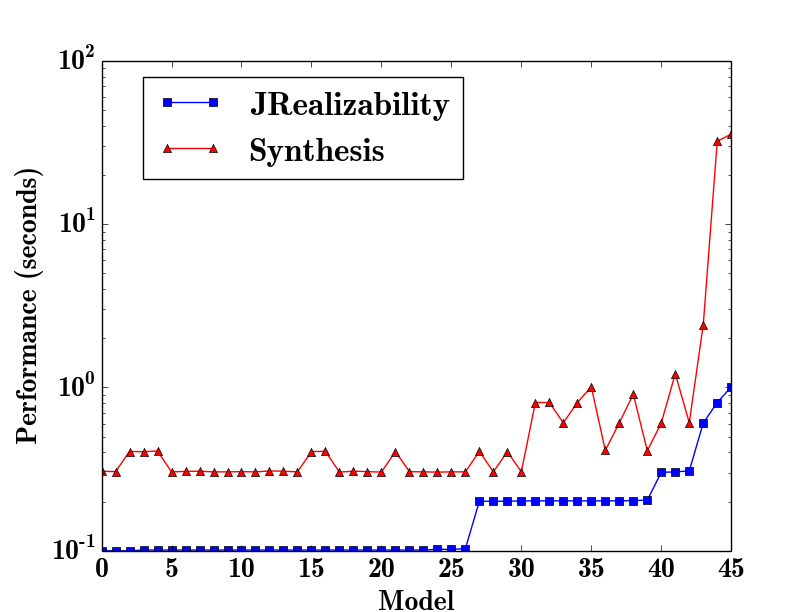
\includegraphics[width=0.4\textwidth,height=\textheight,keepaspectratio]{overhead}\label{fg:overhead}}\hspace{5mm}
	\subfloat[]{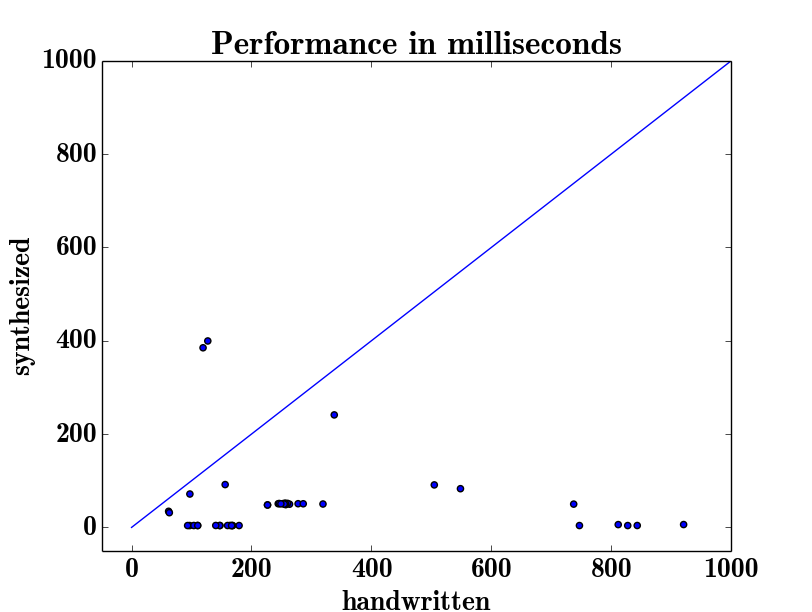
\includegraphics[width=0.4\textwidth,height=\textheight,keepaspectratio]{performance}\label{fg:performance}}\hfill
	\subfloat[]{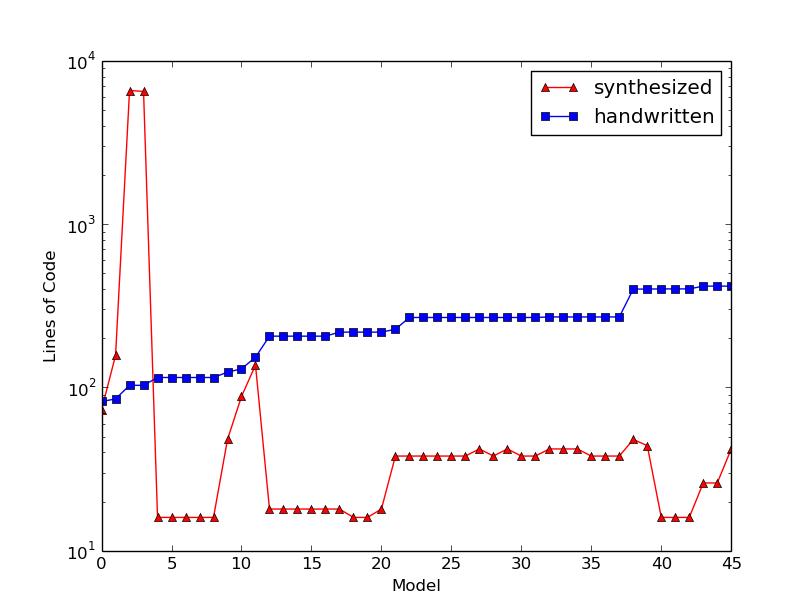
\includegraphics[width=0.4\textwidth,height=\textheight,keepaspectratio]{loc}\label{fg:loc}}    	
	\caption{Experimental results}
	\label{fig:expfigs} 
\end{figure}

Fig.~\ref{fg:overhead} shows the overhead of synthesis by \jkindsynt comparing to the realizability checking by \jkind.
It is at expected levels for the majority of the models. %, with a few outstanding
%exceptions where it has a significant impact to the overall performance.
%A particularly interesting way to improve upon this is by switching to a more
%sophisticated algorithm, where we endorse the core idea of Property Directed
%Reachability in terms of finding a proof of realizability, in conjunction with
%AE-VAL's skolemization procedure.
%
Fig.~\ref{fg:performance} provides a scatter plot of the results of our
experiments in terms of the performance of the synthesized programs against the original, handwritten
implementations. Each dot in the scatter plot represents a pair of
running times (x - the handwritten program, y - synthesized one) of the 46
models.
%, with the x axis being the performance of the handwritten
%program, while the y axis reports the corresponding performance of the
%synthesized implementation.
For the two most complex models in the benchmark
suite, the synthesized implementations underperform when compared to the
programs generated by \lustrev. As the level of complexity decreases, we notice
that both implementations share similar performance levels, and for the most
trivial models in the experiment set, the synthesized programs perform better
with a noticeable gap. We attribute these results mainly due to the
simplicity of the requirements expressed in the majority of the models, as all of
them were proved realizable for $k=0$ by \jkind, except for the running example, which was proved for $k=1$.
It is important at this point to recall the fact that the syntesized
implementations are not equivalent to the handwritten versions, in a similar
fashion to the example used in Section~\ref{sec:example}
% \begin{figure}[]
% 	\centering
% 	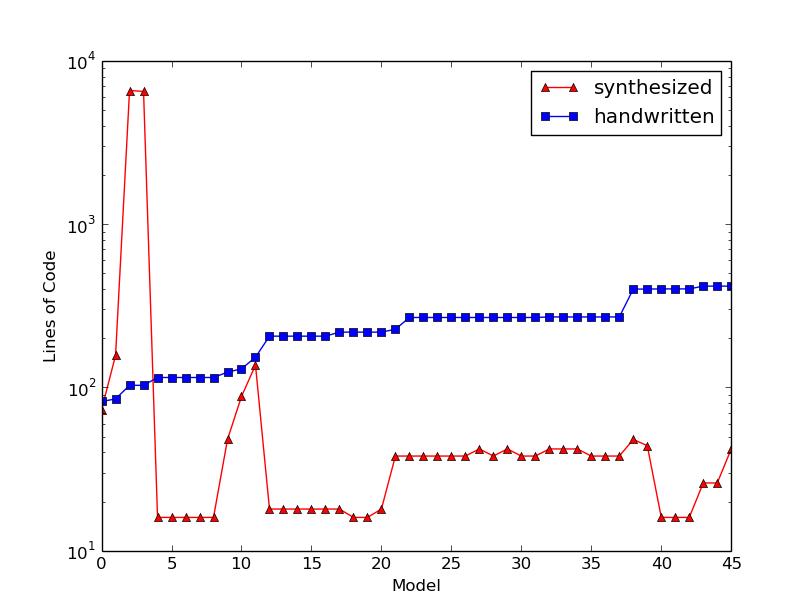
\includegraphics[width=0.6\textwidth,height=\textheight,keepaspectratio]{loc}    	
% 	\caption{Lines of code of synthesized and handwritten implementations}
% 	\label{fg:loc}
% \end{figure}

Fig.~\ref{fg:loc} provides another interesting, as well as important metric in
our experiments, which is the lines of code in each pair of implementations.
Here, we can see the direct effect of the specification complexity to the size
of the Skolem functions generated by \aeval. Two of the three synthesized
programs are also the ones that underperformed their handwritten counterparts in
terms of time. Since the majority of the models contained simple
requirements, the overall size of the synthesized implementation remained well below \lustrev-programs.
%
%For future work, we hope to tackle such cases on three different frontiers. The
%first is again the use of a better algorithm that can effectively reduce the size of
%the transition relation used during the realizability checking algorithm.
%Another interesting idea here is the use of Inductive Validity Cores
%(IVCs)~\cite{Ghass16}, whose main purpose is to effectively pinpoint the
%absolutely necessary model elements in a generated proof. We can potentially use the
%information provided by IVCs as a preprocessing tool to reduce the size of
%the original specification, and hopefully the complexity of the realizability
%proof. Of course, a few optimizations can be further implemented in terms of
%AE-VAL's specific support on proofs of realizability and finally, a very
%important subject is the further improvement of the compiler that we created to
%translate the Skolem functions into C implementations, by introducing
%optimizations like common subexpression elimination.

